% !TEX program = pdflatex
\documentclass[aspectratio=169, 10pt]{beamer}

%% ============================================================
%% PACKAGES
%% ============================================================
\usepackage[T1]{fontenc}
\usepackage{lmodern}
\usepackage{graphicx}
\usepackage{booktabs}
\usepackage{array}
\usepackage{tabularx}
\usepackage{colortbl}
\usepackage{tikz}
\usetikzlibrary{positioning, calc, arrows.meta, shapes.geometric, fit, shadows}
\usepackage[most]{tcolorbox}
\usepackage{fontawesome5}
\usepackage{hyperref}
% appendixnumberbeamer removed (no appendix in this deck)
\usepackage{pgfplots}
\pgfplotsset{compat=1.18}
\usepackage{multicol}
\usepackage{xcolor}
\usepackage{textcomp}
\usepackage{pifont}

\graphicspath{{figures/}}

%% ============================================================
%% COLOR DEFINITIONS
%% ============================================================
\definecolor{UVMGreen}{HTML}{154734}
\definecolor{UVMGold}{HTML}{D4A84B}
\definecolor{SlateTeal}{HTML}{1B4D5C}
\definecolor{DeepCharcoal}{HTML}{2C3E50}
\definecolor{SoftCoral}{HTML}{C0534D}
\definecolor{CoolGray}{HTML}{8899A6}
\definecolor{PaleSage}{HTML}{EDF2F0}
\definecolor{LightGold}{HTML}{FDF6E3}
\definecolor{DarkSlate}{HTML}{0F2B36}
\definecolor{AccentBlue}{HTML}{3498DB}

%% ============================================================
%% BEAMER THEME SETUP
%% ============================================================
\setbeamercolor{structure}{fg=SlateTeal}
\setbeamercolor{normal text}{fg=DeepCharcoal}
\setbeamercolor{frametitle}{fg=SlateTeal}
\setbeamercolor{title}{fg=SlateTeal}
\setbeamercolor{subtitle}{fg=UVMGold}
\setbeamercolor{author}{fg=DeepCharcoal}
\setbeamercolor{date}{fg=CoolGray}
\setbeamercolor{institute}{fg=CoolGray}
\setbeamercolor{footline}{fg=CoolGray}
\setbeamercolor{block title}{fg=white, bg=SlateTeal}
\setbeamercolor{block body}{bg=PaleSage}
\setbeamercolor{alerted text}{fg=SoftCoral}
\setbeamercolor{item}{fg=SlateTeal}
\setbeamercolor{subitem}{fg=CoolGray}

\setbeamerfont{title}{size=\Large, series=\bfseries}
\setbeamerfont{subtitle}{size=\normalsize}
\setbeamerfont{frametitle}{size=\large, series=\bfseries}
\setbeamerfont{footline}{size=\tiny}

\setbeamertemplate{navigation symbols}{}

% Custom frame title
\setbeamertemplate{frametitle}{%
  \vskip14pt%
  \nointerlineskip%
  {\usebeamerfont{frametitle}\usebeamercolor[fg]{frametitle}\insertframetitle\par}%
  \vskip2pt%
  {\color{UVMGold}\rule{\textwidth}{1.2pt}}%
  \vskip3pt%
}

% Custom footline
\setbeamertemplate{footline}{%
  \begin{beamercolorbox}[wd=\paperwidth, ht=16pt, right, rightskip=1.5cm]{footline}%
    \usebeamerfont{footline}\insertframenumber\,/\,\inserttotalframenumber\vskip3pt%
  \end{beamercolorbox}%
}

% Itemize styles
\setbeamertemplate{itemize item}{\color{SlateTeal}\raisebox{0.15ex}{\small$\blacktriangleright$}}
\setbeamertemplate{itemize subitem}{\color{CoolGray}\raisebox{0.1ex}{\footnotesize$\bullet$}}

% Compact tcolorbox defaults
\tcbset{
  keybox/.style={
    colback=PaleSage, colframe=SlateTeal, boxrule=0.8pt, arc=3pt,
    left=6pt, right=6pt, top=4pt, bottom=4pt,
    fonttitle=\bfseries\small\color{white}, coltitle=white, colbacktitle=SlateTeal,
  },
  accentbox/.style={
    colback=LightGold, colframe=UVMGold, boxrule=0.8pt, arc=3pt,
    left=6pt, right=6pt, top=4pt, bottom=4pt,
  },
  quotebox/.style={
    colback=PaleSage, colframe=SlateTeal!50, boxrule=0.5pt, arc=2pt,
    left=8pt, right=8pt, top=4pt, bottom=4pt,
    borderline west={3pt}{0pt}{UVMGold},
  },
}

%% ============================================================
%% METADATA
%% ============================================================
\title{Agentic AI Bootcamp}
\subtitle{From Chat to Autonomous Agents}
\author{Erkmen G. Aslim \and Emily Beam}
\institute{Department of Economics, University of Vermont}
\date{April 22, 2026}

\begin{document}

%% ====== SLIDE 1: TITLE ======
{
\setbeamertemplate{footline}{}
\begin{frame}[plain]
\begin{tikzpicture}[remember picture, overlay]
  % SlateTeal background
  \fill[SlateTeal] (current page.north west) rectangle (current page.south east);
  % Gold accent line across the middle
  \fill[UVMGold] ([yshift=0.3cm]current page.center -| current page.west) rectangle ([yshift=0.25cm]current page.center -| current page.east);
  % Title block (above the line)
  \node[anchor=center, text=white, font=\fontsize{28}{34}\bfseries\selectfont]
    at ([yshift=2.2cm]current page.center) {Agentic AI Bootcamp};
  \node[anchor=center, text=UVMGold, font=\fontsize{15}{20}\selectfont]
    at ([yshift=1.2cm]current page.center) {From Chat to Autonomous Agents};
  % Instructor names (below the line, prominent)
  \node[anchor=center, text=white, font=\large\bfseries]
    at ([yshift=-0.6cm]current page.center) {Erkmen G. Aslim \quad\&\quad Emily Beam};
  \node[anchor=center, text=PaleSage, font=\normalsize]
    at ([yshift=-1.3cm]current page.center) {Department of Economics, University of Vermont};
  % Date and location
  \node[anchor=center, text=CoolGray!70!white, font=\small]
    at ([yshift=-2.2cm]current page.center) {Session 1 \quad$\cdot$\quad April 22, 2026 \quad$\cdot$\quad Old Mill A500};
  \node[anchor=center, text=UVMGold, font=\small\ttfamily]
    at ([yshift=-2.8cm]current page.center) {eabeam.github.io/uvmecon-ai};
  % Subtle robot watermark
  \node[text=white, opacity=0.04, font=\fontsize{100}{100}\selectfont, anchor=center, rotate=-15]
    at ([xshift=5cm, yshift=1.5cm]current page.center) {\faRobot};
\end{tikzpicture}
\end{frame}
}

%% ====== SLIDE 2: AGENDA ======
\begin{frame}{What We'll Cover Today}
\begin{columns}[T]
\begin{column}{0.47\textwidth}
\begin{tcolorbox}[keybox, title={\faMap\quad Concepts}]
\small
\begin{itemize}\setlength{\itemsep}{2pt}
  \item What is agentic AI?
  \item Chat AI vs.\ autonomous agents
  \item The context window
  \item Planning \& markdown files
  \item Permissions \& safety
\end{itemize}
\end{tcolorbox}
\end{column}
\begin{column}{0.47\textwidth}
\begin{tcolorbox}[keybox, title={\faLaptopCode\quad Hands-On}]
\small
\begin{itemize}\setlength{\itemsep}{2pt}
  \item Claude Code vs.\ Codex
  \item Terminal vs.\ Desktop App
  \item Skills: reusable workflows
  \item \textbf{App 1:} Website redesign
  \item \textbf{App 2:} Skill creation
\end{itemize}
\end{tcolorbox}
\end{column}
\end{columns}
\vfill
\begin{center}
\color{CoolGray}\small No prior experience required. Bring curiosity and a task you'd like to automate.
\end{center}
\end{frame}

%% ====== SLIDE 3: AI LADDER ======
\begin{frame}{Where Are You on the AI Ladder?}
\centering
\vskip2pt
{\small
\begin{tabular}{>{\centering\arraybackslash\bfseries}m{1cm} m{12cm}}
\rowcolor{SlateTeal}
\textcolor{white}{Level} & \centering\arraybackslash\textcolor{white}{\textbf{What It Looks Like}} \\[1pt]
\rowcolor{PaleSage}
\textcolor{SlateTeal}{0} & Copy code from ChatGPT in a browser, paste into your editor \\[1pt]
\rowcolor{white}
\textcolor{SlateTeal}{1} & IDE (VS Code, Cursor, Zed) offers inline completions and inline chat \\[1pt]
\rowcolor{PaleSage}
\textcolor{SlateTeal}{2} & ``Agent mode'' inside the IDE: the model can read files, run tests, refactor \\[1pt]
\rowcolor{white}
\textcolor{SlateTeal}{3} & \textbf{Dedicated coding agents} (Claude Code, Codex CLI, \ldots) \\[1pt]
\rowcolor{PaleSage}
\textcolor{SlateTeal}{4} & Attach tools so agents can search the web, scrape, browse, orchestrate \\[1pt]
\rowcolor{white}
\textcolor{SlateTeal}{5} & Orchestrate teams of agents in containers \\[1pt]
\end{tabular}
}
\vskip8pt
\pause
\begin{tcolorbox}[accentbox, width=10cm, halign=center]
\small Most researchers are at \textbf{Level 0--1}. This bootcamp gets you to \textbf{Level 3--4}.
\end{tcolorbox}
\vskip2pt
{\scriptsize\color{CoolGray} Adapted from Paul Goldsmith-Pinkham (2026)}
\end{frame}

%% ====== SLIDE 4: CHAT vs AGENTIC ======
\begin{frame}{Chat AI vs.\ Agentic AI}
\begin{columns}[T]
\begin{column}{0.44\textwidth}
\begin{tcolorbox}[colback=PaleSage, colframe=CoolGray, boxrule=0.6pt, arc=3pt, left=5pt, right=5pt, top=3pt, bottom=3pt, title={\faComments\quad ChatGPT / Claude Web}, fonttitle=\bfseries\scriptsize, coltitle=DeepCharcoal, colbacktitle=PaleSage!80]
\centering
{\scriptsize\color{SoftCoral}\textit{Runs in a sandbox}}
\vskip4pt
\begin{itemize}\small\setlength{\itemsep}{1pt}
  \item Run code snippets
  \item Generate text
  \item[\color{SoftCoral}\faTimes] Can't see your files
  \item[\color{SoftCoral}\faTimes] Can't run commands
\end{itemize}
\end{tcolorbox}
\vskip4pt
\centering
{\scriptsize\color{CoolGray} Like \textbf{texting a smart friend} for advice}
\end{column}
\begin{column}{0.06\textwidth}
\centering\vskip1.2cm
{\large\color{UVMGold}\faArrowRight}
\end{column}
\begin{column}{0.44\textwidth}
\begin{tcolorbox}[colback=LightGold, colframe=UVMGold, boxrule=0.6pt, arc=3pt, left=5pt, right=5pt, top=3pt, bottom=3pt, title={\faTerminal\quad Claude Code / Codex}, fonttitle=\bfseries\scriptsize, coltitle=DeepCharcoal, colbacktitle=LightGold!80]
\centering
{\scriptsize\color{SlateTeal}\textit{Runs on your actual computer}}
\vskip4pt
\begin{itemize}\small\setlength{\itemsep}{1pt}
  \item[\color{SlateTeal}\faCheck] Read \& edit your files
  \item[\color{SlateTeal}\faCheck] Run terminal commands
  \item[\color{SlateTeal}\faCheck] Access your projects
  \item[\color{SlateTeal}\faCheck] Install packages
\end{itemize}
\end{tcolorbox}
\vskip4pt
\centering
{\scriptsize\color{CoolGray} Like having them \textbf{sit next to you}\\and do the work on your computer}
\end{column}
\end{columns}
\end{frame}

%% ====== SLIDE 5: POLL ======
\begin{frame}{Which Agentic Tool Are Economists Using?}
\centering
\vskip2pt
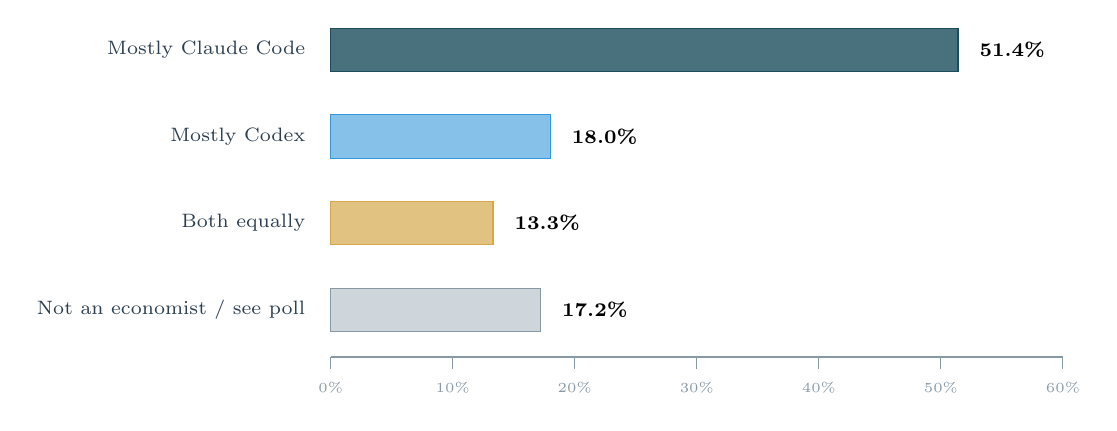
\begin{tikzpicture}[
  barlab/.style={font=\scriptsize, anchor=east, text=DeepCharcoal},
  pctlab/.style={font=\scriptsize\bfseries, anchor=west},
]
  % Y positions
  \def\ya{0}    % Not an economist
  \def\yb{1.1}  % Both equally
  \def\yc{2.2}  % Mostly Codex
  \def\yd{3.3}  % Mostly Claude Code
  \def\bh{0.55} % bar height
  \def\sc{0.155} % scale: 1% = 0.155cm

  % Labels
  \node[barlab] at (-0.2, \yd) {Mostly Claude Code};
  \node[barlab] at (-0.2, \yc) {Mostly Codex};
  \node[barlab] at (-0.2, \yb) {Both equally};
  \node[barlab] at (-0.2, \ya) {Not an economist / see poll};

  % Bars
  \fill[SlateTeal!80] (0, \yd-\bh/2) rectangle ({51.4*\sc}, \yd+\bh/2);
  \draw[SlateTeal] (0, \yd-\bh/2) rectangle ({51.4*\sc}, \yd+\bh/2);

  \fill[AccentBlue!60] (0, \yc-\bh/2) rectangle ({18.0*\sc}, \yc+\bh/2);
  \draw[AccentBlue] (0, \yc-\bh/2) rectangle ({18.0*\sc}, \yc+\bh/2);

  \fill[UVMGold!70] (0, \yb-\bh/2) rectangle ({13.3*\sc}, \yb+\bh/2);
  \draw[UVMGold] (0, \yb-\bh/2) rectangle ({13.3*\sc}, \yb+\bh/2);

  \fill[CoolGray!40] (0, \ya-\bh/2) rectangle ({17.2*\sc}, \ya+\bh/2);
  \draw[CoolGray] (0, \ya-\bh/2) rectangle ({17.2*\sc}, \ya+\bh/2);

  % Percentage labels (all outside bars, same style)
  \node[pctlab] at ({51.4*\sc + 0.15}, \yd) {51.4\%};
  \node[pctlab] at ({18.0*\sc + 0.15}, \yc) {18.0\%};
  \node[pctlab] at ({13.3*\sc + 0.15}, \yb) {13.3\%};
  \node[pctlab] at ({17.2*\sc + 0.15}, \ya) {17.2\%};

  % Axis line
  \draw[CoolGray] (0, -0.6) -- ({60*\sc}, -0.6);
  % Tick marks
  \foreach \v in {0,10,20,30,40,50,60} {
    \draw[CoolGray] ({\v*\sc}, -0.6) -- ({\v*\sc}, -0.75);
    \node[font=\tiny, text=CoolGray, anchor=north] at ({\v*\sc}, -0.8) {\v\%};
  }
\end{tikzpicture}
\vskip4pt
\pause
\begin{tcolorbox}[accentbox, width=12cm, halign=center]
\small The space is evolving fast. \textbf{Our recommendation:} there's value in using \textbf{both}.
\end{tcolorbox}
\vskip1pt
{\tiny\color{CoolGray} Source: @aniketapanjwani poll, X.com --- 459 votes, March 8, 2026}
\end{frame}

%% ====== SLIDE 6: DIVISION OF LABOR ======
\begin{frame}{Division of Labor: Claude Code vs.\ Codex}
\centering
\vskip-2pt
{\small
\begin{tabular}{>{\raggedright\arraybackslash}m{4.5cm} >{\centering\arraybackslash}m{2.8cm} >{\centering\arraybackslash}m{2.8cm}}
\rowcolor{SlateTeal}
\textcolor{white}{\textbf{Task}} & \textcolor{white}{\textbf{Claude Code}} & \textcolor{white}{\textbf{Codex}} \\[2pt]
\rowcolor{PaleSage}
Ideation / brainstorming & \textcolor{SlateTeal}{\faStar\faStar\faStar} & \textcolor{CoolGray}{\faStar} \\[2pt]
\rowcolor{white}
Planning & \textcolor{SlateTeal}{\faStar\faStar} & \textcolor{SlateTeal}{\faStar\faStar} \\[2pt]
\rowcolor{PaleSage}
Review of complex plans & \multicolumn{2}{c}{\textcolor{CoolGray}{\scriptsize ChatGPT \& Claude Pro}} \\[2pt]
\rowcolor{white}
Actual coding / implementation & \textcolor{CoolGray}{\faStar} & \textcolor{SlateTeal}{\faStar\faStar\faStar} \\[2pt]
\rowcolor{PaleSage}
Review of code & \textcolor{SlateTeal}{\faStar\faStar\faStar} & \textcolor{CoolGray}{\faStar} \\[2pt]
\rowcolor{white}
Review of review of code & \textcolor{CoolGray}{\faStar} & \textcolor{SlateTeal}{\faStar\faStar\faStar} \\[2pt]
\rowcolor{PaleSage}
Writing & \textcolor{SlateTeal}{\faStar\faStar\faStar} & \textcolor{CoolGray}{\faStar} \\[2pt]
\rowcolor{white}
OpenClaw & \textcolor{CoolGray}{\faStar} & \textcolor{SlateTeal}{\faStar\faStar\faStar} \\[2pt]
\rowcolor{PaleSage}
Skill creation & \textcolor{SlateTeal}{\faStar\faStar\faStar} & \textcolor{SlateTeal}{\faStar\faStar} \\[2pt]
\end{tabular}
}
\vskip6pt
\pause
\begin{tcolorbox}[quotebox, width=11cm]
\small Think of these tools as \textbf{complementary}, not competing. Use the right tool for the right job.
\end{tcolorbox}
\end{frame}

%% ====== SLIDE 7: PRICING ======
\begin{frame}{Pricing --- What Subscription Do You Need?}
\begin{columns}[T]
\begin{column}{0.47\textwidth}
\begin{tcolorbox}[keybox, title={\faDollarSign\quad Plans}]
\scriptsize
\textbf{Light user} (\$20/mo each):\\
Claude Pro + ChatGPT Plus\\[3pt]
\textbf{Heavy user:}\\
Claude Max: \$100--200/mo\\
ChatGPT Pro: \$200/mo\\[3pt]
\textbf{Pay-as-you-go (API):}\\
Claude Sonnet: \$3--15 per M tokens
\end{tcolorbox}
\end{column}
\begin{column}{0.47\textwidth}
\begin{tcolorbox}[accentbox]
\scriptsize
\textbf{Our recommendation:}
\vskip2pt
Start with the \textbf{\$20/month} plan. Play around before deciding to upgrade.
\vskip4pt
\textbf{Already have ChatGPT?}\\
Codex is included --- no-brainer to try.
\end{tcolorbox}
\vskip4pt
\begin{tcolorbox}[colback=PaleSage, colframe=CoolGray!50, boxrule=0.4pt, left=4pt, right=4pt, top=2pt, bottom=2pt]
\centering\scriptsize
\textbf{What's a token?} 1 token $\approx$ $\frac{3}{4}$ of a word.\\
200K tokens $\approx$ 150K words $\approx$ context limit.
\end{tcolorbox}
\end{column}
\end{columns}
\end{frame}

%% ====== SLIDE 8: CLI vs DESKTOP ======
\begin{frame}{Two Ways to Use It: Terminal vs.\ Desktop App}
\begin{columns}[T]
\begin{column}{0.47\textwidth}
\begin{tcolorbox}[keybox, title={\faTerminal\quad Terminal (CLI)}]
\scriptsize
\begin{itemize}\setlength{\itemsep}{1pt}
  \item Type \texttt{claude} or \texttt{codex}
  \item Gets new features fastest
  \item Lower memory footprint
  \item Power-user flexibility
\end{itemize}
\end{tcolorbox}
\end{column}
\begin{column}{0.47\textwidth}
\begin{tcolorbox}[keybox, title={\faDesktop\quad Desktop App}]
\scriptsize
\begin{itemize}\setlength{\itemsep}{1pt}
  \item Point-and-click interface
  \item More approachable for beginners
  \item Codex app currently more polished
  \item Some report CC app slowdowns
\end{itemize}
\end{tcolorbox}
\end{column}
\end{columns}
\vskip6pt
\pause
\begin{tcolorbox}[quotebox, width=12cm]
\scriptsize I use \textbf{both} terminal and desktop app simultaneously. Think of these as \textbf{different agents} you can deploy on different tasks.
\end{tcolorbox}
\end{frame}

%% ====== SLIDE 9: MULTIPLE AGENTS ======
\begin{frame}[fragile]{Spawning Multiple Agents}
\begin{columns}[T]
\begin{column}{0.42\textwidth}
\vskip2pt
\centering
\begin{tikzpicture}[scale=0.85, every node/.style={scale=0.85},
  agent/.style={
    draw=SlateTeal, fill=PaleSage, rounded corners=3pt,
    minimum width=2.4cm, minimum height=0.75cm, align=center, font=\scriptsize
  },
  task/.style={
    draw=UVMGold, fill=LightGold, rounded corners=2pt,
    minimum width=2.2cm, minimum height=0.45cm, align=center, font=\tiny
  },
  arr/.style={-{Stealth[length=3pt]}, SlateTeal, thick}
]
  \node[draw=SlateTeal, fill=SlateTeal!10, rounded corners=4pt,
        minimum width=2.8cm, minimum height=0.5cm, font=\scriptsize\bfseries]
    (proj) at (0,0) {\faFolder\; Your Project};
  \node[agent, below left=0.6cm and 0.1cm of proj] (a1) {\faTerminal\; Agent 1\\[-1pt](Terminal)};
  \node[agent, below right=0.6cm and 0.1cm of proj] (a2) {\faDesktop\; Agent 2\\[-1pt](Desktop)};
  \node[task, below=0.3cm of a1] (t1) {Lit review + data};
  \node[task, below=0.3cm of a2] (t2) {Slides + figures};
  \draw[arr] (proj.south west) ++(0.2,0) -- (a1.north);
  \draw[arr] (proj.south east) ++(-0.2,0) -- (a2.north);
  \draw[arr] (a1) -- (t1);
  \draw[arr] (a2) -- (t2);
\end{tikzpicture}
\end{column}
\begin{column}{0.52\textwidth}
\vskip2pt
\begin{tcolorbox}[accentbox, top=3pt, bottom=3pt]
\scriptsize
\textbf{The power of parallelism:}
\vskip2pt
\begin{itemize}\setlength{\itemsep}{0pt}\scriptsize
  \item Run multiple agents on \textbf{different tasks} in the same folder
  \item Terminal + desktop app simultaneously
  \item Each agent has its own context window
\end{itemize}
\end{tcolorbox}
\vskip3pt
\pause
\begin{tcolorbox}[quotebox, top=3pt, bottom=3pt]
\scriptsize Like having an \textbf{army of smart RAs} working on different parts of your project at the same time.
\end{tcolorbox}
\end{column}
\end{columns}
\end{frame}

%% ====== SLIDE 10: VOICE MODE ======
\begin{frame}{Voice Mode \& Dictation}
\begin{columns}[T]
\begin{column}{0.47\textwidth}
\begin{tcolorbox}[keybox, title={\faMicrophone\quad Voice in Claude Code}]
\scriptsize
Type \texttt{/voice} to activate hold-to-talk.
\vskip3pt
\begin{itemize}\setlength{\itemsep}{1pt}
  \item Brainstorm ideas hands-free
  \item Draft documents by speaking
  \item Describe complex tasks naturally
\end{itemize}
\end{tcolorbox}
\end{column}
\begin{column}{0.47\textwidth}
\begin{tcolorbox}[keybox, title={\faKeyboard\quad Wispr Flow}]
\scriptsize
System-wide speech-to-text dictation.
\vskip3pt
\begin{itemize}\setlength{\itemsep}{1pt}
  \item Works in any application
  \item Converts speech to polished text
  \item \texttt{wisprflow.ai}
\end{itemize}
\end{tcolorbox}
\end{column}
\end{columns}
\vskip6pt
{\scriptsize\color{CoolGray} Both tools reduce friction when translating thoughts into prompts.}
\end{frame}

%% ====== SLIDE 11: MARKDOWN INTRO ======
\begin{frame}[fragile]{Markdown Files: The Backbone of Agentic AI}
\begin{columns}[T]
\begin{column}{0.50\textwidth}
\vskip2pt
\centering
\begin{tikzpicture}[
  mdfile/.style={
    draw=#1, fill=#1!8, rounded corners=3pt,
    minimum width=4.2cm, minimum height=0.85cm,
    align=left, font=\scriptsize, text=DeepCharcoal
  },
  arr/.style={-{Stealth[length=3pt]}, CoolGray}
]
  \node[mdfile=SlateTeal] (claude) at (0,0)
    {\texttt{CLAUDE.md} / \texttt{AGENTS.md}\\[-1pt]{\tiny\color{CoolGray} Standing rules \& preferences}};
  \node[mdfile=UVMGold, below=0.35cm of claude] (plan)
    {\texttt{PLAN.md}\\[-1pt]{\tiny\color{CoolGray} Strategy \& roadmap}};
  \node[mdfile=AccentBlue, below=0.35cm of plan] (skill)
    {\texttt{SKILL.md}\\[-1pt]{\tiny\color{CoolGray} Reusable playbooks}};
  \node[draw=SlateTeal, fill=SlateTeal, text=white,
        circle, minimum size=0.9cm, font=\scriptsize\bfseries,
        right=1.2cm of plan] (agent) {\faRobot};
  \draw[arr, SlateTeal] (claude.east) -- (agent);
  \draw[arr, UVMGold] (plan.east) -- (agent);
  \draw[arr, AccentBlue] (skill.east) -- (agent);
\end{tikzpicture}
\end{column}
\begin{column}{0.46\textwidth}
\vskip2pt
\begin{tcolorbox}[accentbox]
\scriptsize
\textbf{What are \texttt{.md} files?}
\vskip2pt
Plain text files with simple formatting. They serve as the \textbf{instruction manuals} that guide AI agents.
\vskip3pt
Agents read these to understand:
\begin{itemize}\setlength{\itemsep}{0pt}\tiny
  \item Project rules \& conventions
  \item What to do and how
  \item Your preferred workflows
\end{itemize}
\end{tcolorbox}
\end{column}
\end{columns}
\end{frame}

%% ====== SLIDE 12: CLAUDE.md PITFALLS ======
\begin{frame}[fragile]{\texttt{CLAUDE.md} \& \texttt{AGENTS.md} --- Standing Instructions}
\begin{columns}[T]
\begin{column}{0.46\textwidth}
\begin{tcolorbox}[keybox, title={How They Work}]
\scriptsize
\begin{itemize}\setlength{\itemsep}{1pt}
  \item Loaded \textbf{automatically} at session start
  \item Tell agent: style, do's \& don'ts, conventions
  \item Equivalent of onboarding a new RA
\end{itemize}
\end{tcolorbox}
\vskip3pt
\pause
\begin{tcolorbox}[colback=SoftCoral!8, colframe=SoftCoral, boxrule=0.5pt, left=5pt, right=5pt, top=3pt, bottom=3pt, title={\color{SoftCoral}\faExclamation\; Pitfalls}, fonttitle=\scriptsize\bfseries, coltitle=SoftCoral]
\scriptsize
\begin{enumerate}\setlength{\itemsep}{0pt}
  \item Too much context $\rightarrow$ hurts performance
  \item \texttt{/init} doesn't produce great files
  \item Files go stale quickly
\end{enumerate}
\end{tcolorbox}
\end{column}
\begin{column}{0.50\textwidth}
\begin{tcolorbox}[colback=PaleSage, colframe=SlateTeal!50, boxrule=0.5pt, left=4pt, right=4pt, top=3pt, bottom=3pt]
\centering\scriptsize
\textbf{Do AGENTS.md files actually help?}
\vskip3pt
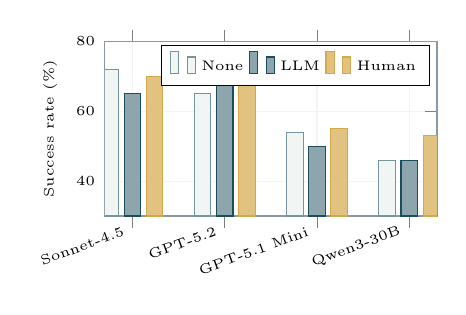
\begin{tikzpicture}
\begin{axis}[
    ybar, bar width=6pt,
    width=5.8cm, height=3.8cm,
    ymin=30, ymax=80,
    ylabel={\tiny Success rate (\%)},
    symbolic x coords={Sonnet-4.5, GPT-5.2, GPT-5.1 Mini, Qwen3-30B},
    xtick=data,
    xticklabel style={font=\tiny, rotate=20, anchor=east},
    yticklabel style={font=\tiny},
    ylabel style={font=\tiny},
    legend style={font=\tiny, at={(0.98,0.98)}, anchor=north east, legend columns=3},
    axis line style={draw=CoolGray},
    grid=major, grid style={draw=CoolGray!12},
]
\addplot[fill=PaleSage!80, draw=SlateTeal!60] coordinates {(Sonnet-4.5,72) (GPT-5.2,65) (GPT-5.1 Mini,54) (Qwen3-30B,46)};
\addplot[fill=SlateTeal!50, draw=SlateTeal] coordinates {(Sonnet-4.5,65) (GPT-5.2,68) (GPT-5.1 Mini,50) (Qwen3-30B,46)};
\addplot[fill=UVMGold!70, draw=UVMGold] coordinates {(Sonnet-4.5,70) (GPT-5.2,68) (GPT-5.1 Mini,55) (Qwen3-30B,53)};
\legend{None, LLM, Human}
\end{axis}
\end{tikzpicture}
\vskip1pt
{\tiny\color{CoolGray} Gloaguen et al.\ (2026), ETH Zurich / INSAIT}
\end{tcolorbox}
\end{column}
\end{columns}
\end{frame}

%% ====== SLIDE 13: CAPABILITY TOOLBELT ======
\begin{frame}[fragile]{The Capability Toolbelt}
\centering
\vskip2pt
\begin{tikzpicture}[scale=0.95, every node/.style={scale=0.95},
  mainbox/.style={
    draw=UVMGold, fill=LightGold, rounded corners=4pt,
    minimum width=10.5cm, minimum height=0.8cm,
    font=\small\bfseries, text=DeepCharcoal
  },
  toolbox/.style={
    draw=CoolGray!60, fill=PaleSage, rounded corners=3pt,
    minimum width=2.2cm, minimum height=1.2cm,
    align=center, font=\scriptsize, text=DeepCharcoal
  },
  arr/.style={-{Stealth[length=3pt]}, CoolGray, thick}
]
  % Four tool boxes
  \node[toolbox] (skills) at (-3.6,-2)
    {{\normalsize\color{SlateTeal}\faCubes}\\[1pt]\textbf{Skills}\\[-1pt]{\tiny Instructions}};
  \node[toolbox, right=0.25cm of skills] (mcps)
    {{\normalsize\color{SlateTeal}\faPlug}\\[1pt]\textbf{MCPs}\\[-1pt]{\tiny Access}};
  \node[toolbox, right=0.25cm of mcps] (plugins)
    {{\normalsize\color{SlateTeal}\faPuzzlePiece}\\[1pt]\textbf{Plugins}\\[-1pt]{\tiny Community}};
  \node[toolbox, right=0.25cm of plugins] (subagents)
    {{\normalsize\color{SlateTeal}\faUsers}\\[1pt]\textbf{Subagents}\\[-1pt]{\tiny Scale}};
  % CLI box centered above the four tool boxes
  \path (skills.north) -- (subagents.north) coordinate[midway] (toolmid);
  \node[mainbox] (cli) at ([yshift=0.9cm]toolmid) {\faTerminal\quad CLI --- You talk to Claude; it uses tools on your machine};
  % Arrows
  \draw[arr] (cli.south -| skills) -- (skills.north);
  \draw[arr] (cli.south -| mcps) -- (mcps.north);
  \draw[arr] (cli.south -| plugins) -- (plugins.north);
  \draw[arr] (cli.south -| subagents) -- (subagents.north);
\end{tikzpicture}
\vskip6pt
\pause
\begin{tcolorbox}[quotebox, width=10cm]
\scriptsize Today we focus on \textbf{Skills}. MCPs and plugins are powerful but outside the scope of this bootcamp.
\end{tcolorbox}
\vskip1pt
{\tiny\color{CoolGray} Adapted from Aniket Panjwani's Claude Code course}
\end{frame}

%% ====== SLIDE 14: CONTEXT WINDOW ======
\begin{frame}{The Context Window --- The Key Concept}
\begin{columns}[T]
\begin{column}{0.47\textwidth}
\begin{tcolorbox}[keybox, title={What the model ``sees''}]
\scriptsize
\begin{itemize}\setlength{\itemsep}{0pt}
  \item System prompt
  \item Developer messages (tools)
  \item Your prompt + model's ``thinking''
  \item Tool calls \& results
  \item Model's response
  \item \ldots all appended each turn
\end{itemize}
\end{tcolorbox}
\end{column}
\begin{column}{0.47\textwidth}
\begin{tcolorbox}[accentbox]
\scriptsize
\textbf{Every turn:} the entire history gets sent as one input.
\vskip4pt
\textbf{Limit:} $\sim$200K tokens ($\sim$150K words)
\end{tcolorbox}
\vskip4pt
\pause
\begin{tcolorbox}[colback=SoftCoral!8, colframe=SoftCoral, boxrule=0.5pt, left=5pt, right=5pt, top=3pt, bottom=3pt]
\centering\scriptsize
This is the \textbf{single most important concept} for using these tools well.
\end{tcolorbox}
\end{column}
\end{columns}
\end{frame}

%% ====== SLIDE 15: WHY CONTEXT MATTERS ======
\begin{frame}[fragile]{Why the Context Window Matters}
\centering
\vskip2pt
\begin{tcolorbox}[colback=PaleSage, colframe=SlateTeal, boxrule=0.6pt, width=7cm, halign=center, top=3pt, bottom=3pt]
\normalsize
$\text{Performance} \;\approx\; \dfrac{\text{correctness}^2 \times \text{completeness}}{\text{size}}$
\end{tcolorbox}
\vskip6pt
\begin{columns}[T]
\begin{column}{0.47\textwidth}
\scriptsize
\begin{itemize}\setlength{\itemsep}{2pt}
  \item As context grows $\rightarrow$ performance \textbf{degrades}
  \item More files, history, outputs $\rightarrow$ model loses the thread
\end{itemize}
\end{column}
\begin{column}{0.47\textwidth}
\begin{tcolorbox}[accentbox, top=3pt, bottom=3pt]
\scriptsize
\textbf{Context engineering} is the new prompt engineering. It's not just what you say --- it's what's \textit{in} the window.
\end{tcolorbox}
\end{column}
\end{columns}
\vskip6pt
\pause
% Compaction diagram
\centering
\begin{tikzpicture}[
  bigbox/.style={draw=SlateTeal, rounded corners=3pt, minimum width=3cm, font=\tiny, align=center},
]
  \node[bigbox, fill=SoftCoral!12, minimum height=1.6cm] (before) at (0,0) {};
  \node[font=\tiny\bfseries, above=0pt of before.north, anchor=south] {Before Compaction};
  \node[font=\tiny, text=CoolGray] at (0,0.35) {Messages + files + tools};
  \node[font=\tiny, text=SoftCoral] at (0,-0.15) {\textit{Nearly full!}};
  \node[font=\normalsize, text=UVMGold] at (2.2,0) {\faArrowRight};
  \node[bigbox, fill=PaleSage, minimum height=1.6cm] (after) at (4.4,0) {};
  \node[font=\tiny\bfseries, above=0pt of after.north, anchor=south] {After Compaction};
  \node[font=\tiny, text=SlateTeal] at (4.4,0.35) {Summary + key decisions};
  \node[font=\tiny, text=CoolGray] at (4.4,-0.15) {Free space for new work};
\end{tikzpicture}
\end{frame}

%% ====== SLIDE 16: THREE RULES ======
\begin{frame}{Three Rules for Context Management}
\begin{columns}[T]
\begin{column}{0.55\textwidth}
\vskip2pt
\begin{enumerate}\setlength{\itemsep}{6pt}
  \item[\color{SlateTeal}\textbf{1.}] \textbf{Long sessions degrade} --- after 20+ turns, start fresh
  \pause
  \item[\color{SlateTeal}\textbf{2.}] \textbf{Write ideas to files} --- files persist, context doesn't
  \pause
  \item[\color{SlateTeal}\textbf{3.}] \textbf{Break work into chunks} --- 5--10 turn focused sessions
\end{enumerate}
\vskip8pt
\begin{tcolorbox}[quotebox]
\scriptsize \textbf{Frequent intentional compaction is better} than hitting the wall and letting auto-compaction lose details.
\end{tcolorbox}
\end{column}
\begin{column}{0.42\textwidth}
\vskip2pt
\begin{tcolorbox}[accentbox]
\scriptsize
\textbf{The ``start fresh'' pattern:}
\vskip2pt
\begin{enumerate}\setlength{\itemsep}{0pt}\tiny
  \item Write progress to \texttt{PLAN.md}
  \item Start a new session
  \item ``Read \texttt{PLAN.md} and continue\ldots''
  \item Full context budget restored!
\end{enumerate}
\end{tcolorbox}
\vskip4pt
{\tiny\color{CoolGray} Recent Opus 4.6 improvements mean this matters less --- but still good practice.}
\end{column}
\end{columns}
\end{frame}

%% ====== SLIDE 17: PERMISSION MODES ======
\begin{frame}[fragile]{Permission Modes}
\centering
\vskip2pt
\begin{tikzpicture}[
  modebox/.style={
    draw=#1, fill=#1!8, rounded corners=4pt,
    minimum width=2.6cm, minimum height=1.8cm,
    align=center, font=\scriptsize, text=DeepCharcoal
  },
]
  \node[modebox=SlateTeal] (default) at (0,0)
    {{\normalsize\color{SlateTeal}\faLock}\\[2pt]\textbf{Default}\\[-1pt]{\tiny Prompts on first use}};
  \node[modebox=AccentBlue, right=0.3cm of default] (accept)
    {{\normalsize\color{AccentBlue}\faEdit}\\[2pt]\textbf{Accept Edits}\\[-1pt]{\tiny Auto-approves edits}};
  \node[modebox=UVMGold, right=0.3cm of accept] (plan)
    {{\normalsize\color{UVMGold}\faClipboard}\\[2pt]\textbf{Plan Mode}\\[-1pt]{\tiny Read-only}};
  \node[modebox=SoftCoral, right=0.3cm of plan] (yolo)
    {{\normalsize\color{SoftCoral}\faBolt}\\[2pt]\textbf{YOLO}\\[-1pt]{\tiny Skips all prompts}};
  \draw[-{Stealth[length=3pt]}, CoolGray, thick, bend left=18] (default.north) to node[above, font=\tiny\color{CoolGray}] {Shift+Tab} (accept.north);
  \draw[-{Stealth[length=3pt]}, CoolGray, thick, bend left=18] (accept.north) to (plan.north);
  \draw[-{Stealth[length=3pt]}, CoolGray, thick, bend left=18] (plan.north) to (yolo.north);
\end{tikzpicture}
\vskip8pt
\pause
\begin{columns}[T]
\begin{column}{0.47\textwidth}
\begin{tcolorbox}[colback=SoftCoral!6, colframe=SoftCoral!50, boxrule=0.4pt, left=5pt, right=5pt, top=2pt, bottom=2pt]
\scriptsize \textbf{YOLO mode:} \texttt{/update-config} $\rightarrow$ set bypass permissions $\rightarrow$ restart.
\end{tcolorbox}
\end{column}
\begin{column}{0.47\textwidth}
\begin{tcolorbox}[colback=PaleSage, colframe=SlateTeal!30, boxrule=0.4pt, left=5pt, right=5pt, top=2pt, bottom=2pt]
\scriptsize \textbf{Fine-grained:} \texttt{/permissions} to see allow/ask/deny rules.
\end{tcolorbox}
\end{column}
\end{columns}
\end{frame}

%% ====== SLIDE 18: SAFETY + BEST PRACTICES ======
\begin{frame}{Safety Nets \& Best Practices}
\begin{columns}[T]
\begin{column}{0.44\textwidth}
\begin{tcolorbox}[keybox, title={\faLock\quad Safety}]
\scriptsize
\textbf{Destructive Command Guard:}\\
Hooks that block dangerous commands (\texttt{rm -rf /}) before execution.
\vskip3pt
Hooks are powerful --- but \textbf{outside the scope} of this bootcamp.
\end{tcolorbox}
\end{column}
\begin{column}{0.52\textwidth}
\begin{tcolorbox}[keybox, title={\faLightbulb\quad Four Prompting Rules}]
\scriptsize
\begin{enumerate}\setlength{\itemsep}{1pt}
  \item \textbf{Be specific.}
    {\tiny Not ``analyze data'' but ``load employment.csv, compute growth rates.''}
  \item \textbf{Iterate, don't argue.}
    {\tiny Going in circles? Hit ESC, start over.}
  \item \textbf{Correct early.}
    {\tiny Catch wrong foundations immediately.}
  \item \textbf{Trust but verify.}
    {\tiny Mistakes happen with edge cases.}
\end{enumerate}
\end{tcolorbox}
\end{column}
\end{columns}
\end{frame}

%% ====== SLIDE 19: POWER OF PLANNING ======
\begin{frame}[fragile]{The Power of Planning (\texttt{PLAN.md})}
\begin{columns}[T]
\begin{column}{0.52\textwidth}
\begin{tcolorbox}[quotebox, top=3pt, bottom=3pt]
\scriptsize I spend most of my time \textbf{planning}, especially for complex multi-step projects.
\end{tcolorbox}
\vskip3pt
\centering
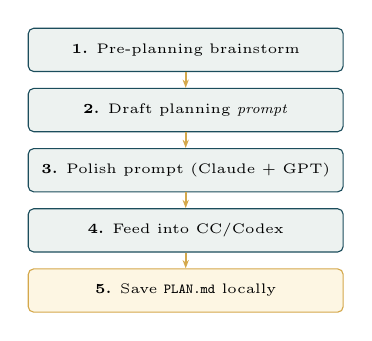
\begin{tikzpicture}[
  planstep/.style={
    draw=SlateTeal, fill=PaleSage, rounded corners=2pt,
    minimum width=4cm, minimum height=0.55cm,
    align=center, font=\tiny
  },
  arr/.style={-{Stealth[length=3pt]}, UVMGold, thick}
]
  \node[planstep] (s1) at (0,0) {\textbf{1.} Pre-planning brainstorm};
  \node[planstep, below=0.2cm of s1] (s2) {\textbf{2.} Draft planning \textit{prompt}};
  \node[planstep, below=0.2cm of s2] (s3) {\textbf{3.} Polish prompt (Claude + GPT)};
  \node[planstep, below=0.2cm of s3] (s4) {\textbf{4.} Feed into CC/Codex};
  \node[planstep, below=0.2cm of s4, fill=LightGold, draw=UVMGold] (s5) {\textbf{5.} Save \texttt{PLAN.md} locally};
  \draw[arr] (s1) -- (s2);
  \draw[arr] (s2) -- (s3);
  \draw[arr] (s3) -- (s4);
  \draw[arr] (s4) -- (s5);
\end{tikzpicture}
\end{column}
\begin{column}{0.44\textwidth}
\vskip2pt
\begin{tcolorbox}[accentbox, top=3pt, bottom=3pt]
\scriptsize
\textbf{What goes in a plan?}
\begin{itemize}\setlength{\itemsep}{0pt}\tiny
  \item Project objectives
  \item Do's and don'ts
  \item Inputs and outputs
  \item Lessons from prior projects
\end{itemize}
\end{tcolorbox}
\vskip3pt
\begin{tcolorbox}[colback=PaleSage, colframe=SlateTeal!40, boxrule=0.4pt, left=4pt, right=4pt, top=2pt, bottom=2pt]
\scriptsize
\textbf{Why save locally?}\\
Every fresh context starts with:\\
\texttt{``Read PLAN.md and continue...''}
\end{tcolorbox}
\end{column}
\end{columns}
\end{frame}

%% ====== SLIDE 20: WHY PLANNING PAYS OFF ======
\begin{frame}{Why Planning Pays Off}
\centering
\vskip2pt
\begin{tcolorbox}[accentbox, width=12cm, halign=center, top=3pt, bottom=3pt]
\normalsize\bfseries Upstream planning impacts downstream outcomes.
\end{tcolorbox}
\vskip6pt
\begin{columns}[T]
\begin{column}{0.46\textwidth}
\begin{tcolorbox}[keybox, title={Without a plan}]
\scriptsize
\begin{itemize}\setlength{\itemsep}{1pt}
  \item Constant back-and-forth fixing
  \item Wasted tokens on corrections
  \item Agent builds on wrong foundation
\end{itemize}
\end{tcolorbox}
\end{column}
\begin{column}{0.46\textwidth}
\begin{tcolorbox}[keybox, title={With a detailed plan}]
\scriptsize
\begin{itemize}\setlength{\itemsep}{1pt}
  \item Reduces or \textbf{eliminates} rework
  \item Fewer tokens $\rightarrow$ lower cost
  \item Multiple sessions stay aligned
\end{itemize}
\end{tcolorbox}
\end{column}
\end{columns}
\vskip6pt
\pause
\begin{tcolorbox}[quotebox, width=11cm]
\scriptsize A detailed plan will save you a \textbf{TON} of time. Think long-term gains, not short term. May not matter for quick tasks!
\end{tcolorbox}
\end{frame}

%% ====== SLIDE 21: WHAT ARE SKILLS ======
\begin{frame}{What Are Skills?}
\begin{columns}[T]
\begin{column}{0.46\textwidth}
\begin{tcolorbox}[keybox, title={\faCubes\quad Definition}]
\scriptsize
Markdown instruction \textbf{playbooks} that teach Claude Code how to perform a specific task consistently.
\vskip3pt
Think of them as \textbf{SOPs for your AI agent}.
\vskip3pt
\textbf{Invoke:} \texttt{/skill-name}\\
\textbf{Browse:} \texttt{/skills}\\
\textbf{Create:} \texttt{/skill-creator}
\end{tcolorbox}
\end{column}
\begin{column}{0.46\textwidth}
\begin{tcolorbox}[colback=PaleSage, colframe=SlateTeal!50, boxrule=0.4pt, left=5pt, right=5pt, top=3pt, bottom=3pt]
\scriptsize
\textbf{Why not just prompt every time?}
\vskip3pt
\begin{tabular}{@{}l@{\;}c@{\;}c@{}}
 & \textbf{Prompt} & \textbf{Skill} \\
\midrule
Consistency & \textcolor{SoftCoral}{Low} & \textcolor{SlateTeal}{High} \\
Quality & \textcolor{CoolGray}{Variable} & \textcolor{SlateTeal}{High} \\
Token use & \textcolor{SoftCoral}{Higher} & \textcolor{SlateTeal}{Lower} \\
Reusable & \textcolor{SoftCoral}{No} & \textcolor{SlateTeal}{Yes} \\
\end{tabular}
\end{tcolorbox}
\vskip3pt
{\tiny\color{CoolGray} Advanced skills can include Python scripts and supporting files.}
\end{column}
\end{columns}
\end{frame}

%% ====== SLIDE 22: INSTALLING SKILLS ======
\begin{frame}{Installing Anthropic Skills}
\begin{columns}[T]
\begin{column}{0.52\textwidth}
\begin{tcolorbox}[keybox, title={\faDownload\quad Step-by-Step}]
\scriptsize
\textbf{1. Add the marketplace:}\\
\texttt{/plugin marketplace add anthropics/skills}
\vskip4pt
\textbf{2. Install a skill set:}\\
\texttt{/plugin install}\\
\texttt{\; document-skills@anthropic-agent-skills}
\vskip4pt
\textbf{3. Use it:}\\
\texttt{/frontend-design} \; \texttt{/pdf} \; \texttt{/docx}
\end{tcolorbox}
\end{column}
\begin{column}{0.44\textwidth}
\vskip2pt
\begin{tcolorbox}[accentbox]
\scriptsize
\textbf{Also available:}
\begin{itemize}\setlength{\itemsep}{0pt}\tiny
  \item \texttt{/find-data} --- dataset discovery
  \item \texttt{/lit-review} --- literature synthesis
  \item \texttt{/econ-audit} --- empirical review
  \item \texttt{/pptx} --- PowerPoint creation
  \item \texttt{/xlsx} --- spreadsheet tools
\end{itemize}
\end{tcolorbox}
\vskip3pt
{\tiny\color{CoolGray} Browse community skills at \texttt{skills.sh}}
\end{column}
\end{columns}
\end{frame}

%% ====== SLIDE 23: BREADTH OF SKILLS ======
\begin{frame}[fragile]{The Breadth of Possible Skills}
\centering
\vskip2pt
\begin{tikzpicture}[
  card/.style={
    draw=CoolGray!40, fill=white, rounded corners=3pt,
    minimum width=4.2cm, minimum height=1.1cm,
    align=left, font=\scriptsize, text=DeepCharcoal
  }
]
  \node[font=\small\bfseries, text=SlateTeal] at (-2.8,2.1) {\faChalkboard\quad Teaching};
  \node[card] at (-2.8,1.2) {\faBook\; Lecture notes \& slides\\[-1pt]{\tiny from papers, textbooks, blogs}};
  \node[card] at (-2.8,0) {\faCheck\; Assignment feedback\\[-1pt]{\tiny \& automated grading}};
  \node[card] at (-2.8,-1.2) {\faDatabase\; Pseudo data generation\\[-1pt]{\tiny Stata, R, Python examples}};

  \node[font=\small\bfseries, text=UVMGold] at (2.8,2.1) {\faSearch\quad Research};
  \node[card] at (2.8,1.2) {\faSearch\; Data discovery\\[-1pt]{\tiny across repositories \& APIs}};
  \node[card] at (2.8,0) {\faFile\; Literature review\\[-1pt]{\tiny \& evidence synthesis}};
  \node[card] at (2.8,-1.2) {\faGlobe\; Web scraping\\[-1pt]{\tiny pipelines (Session 2!)}};
\end{tikzpicture}
\vskip6pt
\pause
\begin{tcolorbox}[quotebox, width=10cm]
\scriptsize If you repeat a workflow more than twice, it should probably be a skill.
\end{tcolorbox}
\end{frame}

%% ====== SECTION DIVIDER: APP 1 ======
{
\setbeamertemplate{footline}{}
\begin{frame}[plain, noframenumbering]
\begin{tikzpicture}[remember picture, overlay]
  \fill[SlateTeal] (current page.north west) rectangle (current page.south east);
  \node[text=white, font=\fontsize{22}{28}\bfseries\selectfont]
    at ([yshift=0.4cm]current page.center) {Application 1};
  \node[text=UVMGold, font=\normalsize]
    at ([yshift=-0.4cm]current page.center) {Website Redesign with \texttt{/frontend-design}};
  \draw[UVMGold, line width=0.8pt] ([xshift=-2.5cm, yshift=0cm]current page.center) -- ([xshift=2.5cm, yshift=0cm]current page.center);
\end{tikzpicture}
\end{frame}
}

%% ====== APP 1 OVERVIEW ======
\begin{frame}{Application 1: Redesigning a Faculty Website}
\begin{columns}[T]
\begin{column}{0.50\textwidth}
\begin{tcolorbox}[keybox, title={\faGlobe\quad The Task}]
\scriptsize
Take an existing faculty website and redesign it using \texttt{/frontend-design}.
\vskip3pt
\textbf{Target:} \texttt{erkmengirayaslim.com}\\
\textbf{Inspiration:} Anthropic's site + Caitlin Myers's site\\
\textbf{Output:} HTML + screenshots, saved locally.\\
We are \textit{not} launching --- just demonstrating.
\end{tcolorbox}
\end{column}
\begin{column}{0.44\textwidth}
\vskip2pt
\begin{tcolorbox}[accentbox]
\scriptsize
\textbf{Why this demo?}
\begin{itemize}\setlength{\itemsep}{0pt}\tiny
  \item Shows power of a single skill
  \item Tangible result in minutes
  \item Demonstrates prompt specificity
  \item Faculty can immediately relate
\end{itemize}
\end{tcolorbox}
\vskip3pt
{\scriptsize\color{CoolGray} \faPlay\; Live demo runs in background.}
\end{column}
\end{columns}
\end{frame}

%% ====== APP 1 PROMPT ======
\begin{frame}{The Prompt}
\begin{tcolorbox}[colback=DarkSlate, colframe=DarkSlate, arc=3pt, left=8pt, right=8pt, top=6pt, bottom=6pt]
{\color{CoolGray}\ttfamily\tiny /frontend-design\\[2pt]
\color{white}\scriptsize
I have a website at erkmengirayaslim.com. Please redesign it with a modern, clean aesthetic. Use anthropic.com for design inspiration (minimal, spacious) and caitlinmyers.github.io for academic content structure.\\[3pt]
Create three distinct mock-ups:\\
1. Minimal dark theme with accent colors\\
2. Light academic theme with card-based layout\\
3. Bold modern theme with full-width hero sections\\[3pt]
Download all content from my current site. Save HTML files and screenshot PNGs to the current directory.\\[3pt]
Focus on: clean typography, clear navigation, prominent research section, responsive design.
}
\end{tcolorbox}
\vskip4pt
\begin{tcolorbox}[quotebox, width=12cm]
\scriptsize Notice how the prompt is \textbf{specific}: skill name, target, inspiration, number of outputs, where to save. This is effective prompting.
\end{tcolorbox}
\end{frame}

%% ====== APP 1 RESULTS ======
\begin{frame}[fragile]{The Results}
\centering
\vskip4pt
\begin{tcolorbox}[accentbox, width=11cm, halign=center, top=3pt, bottom=3pt]
\normalsize \faLaptopCode\quad Live Demo --- Results Appearing in Real Time
\end{tcolorbox}
\vskip8pt
\begin{tikzpicture}[
  mock/.style={
    draw=CoolGray!50, fill=PaleSage!30, rounded corners=3pt,
    minimum width=3.2cm, minimum height=3.5cm, align=center, font=\scriptsize
  }
]
  \node[mock] (m1) at (0,0) {{\large\color{SlateTeal}\faMoon}\\[4pt]\textbf{Mock-up 1}\\{\tiny Minimal dark theme}};
  \node[mock] (m2) at (4,0) {{\large\color{UVMGold}\faSun}\\[4pt]\textbf{Mock-up 2}\\{\tiny Light academic theme}};
  \node[mock] (m3) at (8,0) {{\large\color{SoftCoral}\faPalette}\\[4pt]\textbf{Mock-up 3}\\{\tiny Bold modern theme}};
\end{tikzpicture}
\vskip8pt
{\small\color{CoolGray} One prompt. Three complete website redesigns. $\sim$2--5 minutes.}
\end{frame}

%% ====== APP 1 EXAMPLE OUTPUT ======
\begin{frame}{The Results --- A Real Example}
\centering
\vskip4pt
\begin{tcolorbox}[accentbox, width=11cm, halign=center, top=3pt, bottom=3pt]
\normalsize \faLaptopCode\quad Mock-up 3: Bold Modern Theme --- Actual Output
\end{tcolorbox}
\vskip6pt
\includegraphics[width=0.45\textwidth, keepaspectratio]{figures/website-ea.png}
\vskip6pt
{\small\color{CoolGray} Dark hero, full-width layout (suitable for web \& mobile browsers) --- generated in a single session.}
\end{frame}

%% ====== ANATOMY OF A SKILL (moved before App 2) ======
\begin{frame}[fragile]{Anatomy of a Skill}
\centering
\vskip2pt
\begin{tikzpicture}[
  filebox/.style={
    draw=#1, fill=#1!8, rounded corners=2pt,
    minimum width=5cm, minimum height=0.7cm,
    align=left, font=\scriptsize\ttfamily, text=DeepCharcoal
  },
  arr/.style={-{Stealth[length=3pt]}, CoolGray}
]
  \node[font=\small\bfseries, text=SlateTeal] at (0,2.4) {\faFolder\; \texttt{.claude/commands/lecture-builder/}};
  \node[filebox=SlateTeal] (skill) at (0,1.6) {\; SKILL.md {\normalfont\tiny\color{CoolGray} --- instruction playbook}};
  \node[filebox=UVMGold] (parse) at (0,0.7) {\; parse\_document.py {\normalfont\tiny\color{CoolGray} --- PDF/DOCX reader}};
  \node[filebox=AccentBlue] (template) at (0,-0.2) {\; slide\_template.md {\normalfont\tiny\color{CoolGray} --- output format}};
  \node[draw=CoolGray!40, fill=PaleSage, rounded corners=3pt,
        minimum width=4.5cm, minimum height=2.2cm, align=left, font=\scriptsize,
        anchor=west] (desc) at (5.5,0.7) {
    \textbf{SKILL.md contains:}\\[2pt]
    {\tiny $\bullet$ When to trigger}\\
    {\tiny $\bullet$ Step-by-step workflow}\\
    {\tiny $\bullet$ Quality checks}\\
    {\tiny $\bullet$ Output specifications}\\
    {\tiny $\bullet$ Error handling rules}
  };
  \draw[arr] (skill.east) -- ++(0.3,0) |- (desc.west);
\end{tikzpicture}
\vskip8pt
\begin{tcolorbox}[quotebox, width=11cm]
\scriptsize Skills created in Claude Code can be \textbf{copied into Codex} --- they're just markdown files. Write once, use everywhere.
\end{tcolorbox}
\end{frame}

%% ====== SECTION DIVIDER: APP 2 ======
{
\setbeamertemplate{footline}{}
\begin{frame}[plain, noframenumbering]
\begin{tikzpicture}[remember picture, overlay]
  \fill[SlateTeal] (current page.north west) rectangle (current page.south east);
  \node[text=white, font=\fontsize{22}{28}\bfseries\selectfont]
    at ([yshift=0.4cm]current page.center) {Application 2};
  \node[text=UVMGold, font=\normalsize]
    at ([yshift=-0.4cm]current page.center) {Creating a Custom Skill with \texttt{/skill-creator}};
  \draw[UVMGold, line width=0.8pt] ([xshift=-2.5cm, yshift=0cm]current page.center) -- ([xshift=2.5cm, yshift=0cm]current page.center);
\end{tikzpicture}
\end{frame}
}

%% ====== APP 2: LECTURE BUILDER OVERVIEW ======
\begin{frame}{Application 2: Building a ``Lecture Builder'' Skill}
\begin{columns}[T]
\begin{column}{0.47\textwidth}
\begin{tcolorbox}[keybox, title={\faCubes\quad The Goal}]
\scriptsize
Create a skill that:
\begin{enumerate}\setlength{\itemsep}{1pt}
  \item Reads papers, textbooks, articles
  \item Extracts key concepts
  \item Generates structured lecture notes
  \item Produces a polished slide deck
\end{enumerate}
\vskip2pt
\textbf{Invoke with:} \texttt{/lecture-builder}
\end{tcolorbox}
\end{column}
\begin{column}{0.47\textwidth}
\begin{tcolorbox}[accentbox]
\scriptsize
\textbf{Why this is powerful:}
\begin{itemize}\setlength{\itemsep}{0pt}\tiny
  \item 50-page paper $\rightarrow$ 20-slide deck
  \item Consistent formatting every time
  \item Customizable to your teaching style
  \item Sharable with colleagues
\end{itemize}
\end{tcolorbox}
\vskip3pt
{\tiny\color{CoolGray} Advanced skills can include Python scripts (e.g., document parsing), not just markdown.}
\end{column}
\end{columns}
\end{frame}

%% ====== APP 2: SKILL CREATION PROMPT ======
\begin{frame}{The Skill Creation Prompt}
\begin{tcolorbox}[colback=DarkSlate, colframe=DarkSlate, arc=3pt, left=6pt, right=6pt, top=4pt, bottom=4pt]
{\color{CoolGray}\ttfamily\tiny /skill-creator\\[2pt]
\color{white}\tiny
Create a skill called ``lecture-builder'' that converts academic documents into lecture materials. The skill should:\\[1pt]
1. Read documents in their entirety (PDF, DOCX, web pages) --- break reading into parts if needed to avoid excessive token usage. Include a Python parsing script.\\[1pt]
2. Extract: key arguments, empirical findings, methodological details, discussion points, and potential exam questions.\\[1pt]
3. Generate two outputs:\\
\quad a) Structured lecture notes (markdown) with section headers, key takeaways, discussion prompts\\
\quad b) A polished slide deck (draw on /academic-beamer-deck or /pptx) with clean visuals, one idea per slide\\[1pt]
4. Adapt tone for undergraduate vs.\ graduate audiences (configurable).\\[1pt]
Save SKILL.md + all supporting files to .claude/commands/lecture-builder/.
}
\end{tcolorbox}
\vskip4pt
\begin{tcolorbox}[quotebox, width=11cm]
\scriptsize Note the \textbf{detail}: specific inputs, outputs, supporting scripts, and where to save. Effective skill creation prompts mirror effective planning.
\end{tcolorbox}
\end{frame}

%% ====== SLIDE 32: MORE SKILLS ======
\begin{frame}{More Skills to Explore}
\begin{columns}[T]
\begin{column}{0.47\textwidth}
\begin{tcolorbox}[keybox, title={\faChalkboard\quad Teaching Skills}]
\scriptsize
\begin{itemize}\setlength{\itemsep}{1pt}
  \item \texttt{/find-data} --- discover datasets
  \item \texttt{/referee-report-grader} --- grade student reports with rubric
  \item \textbf{Pseudo-data generator} --- Stata, R, Python exercises
\end{itemize}
\end{tcolorbox}
\end{column}
\begin{column}{0.47\textwidth}
\begin{tcolorbox}[keybox, title={\faSearch\quad Research Skills}]
\scriptsize
\begin{itemize}\setlength{\itemsep}{1pt}
  \item \texttt{/lit-review} --- literature synthesis
  \item \texttt{/econ-audit} --- adversarial empirical review
  \item \textbf{Web scraper} --- data collection (Session~2!)
\end{itemize}
\end{tcolorbox}
\end{column}
\end{columns}
\vskip8pt
\begin{tcolorbox}[accentbox, halign=center, width=8cm, top=3pt, bottom=3pt]
\small\bfseries Execution of these skills $\rightarrow$ Session 2
\end{tcolorbox}
\end{frame}

%% ====== SLIDE 33: RECAP ======
\begin{frame}{What We Learned Today}
\centering
\vskip4pt
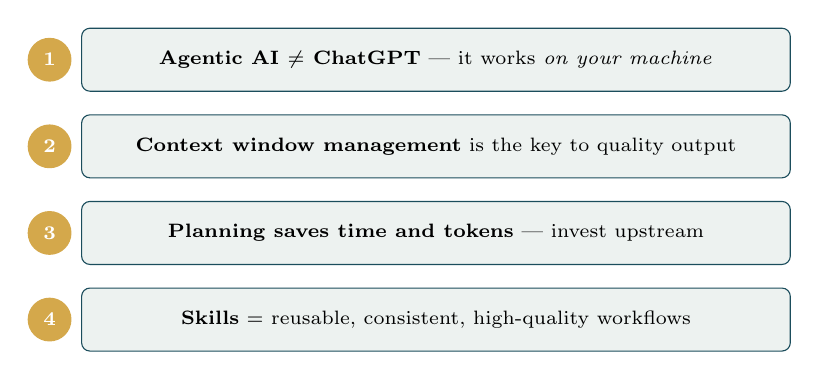
\begin{tikzpicture}[
  takeaway/.style={
    draw=SlateTeal, fill=PaleSage, rounded corners=3pt,
    minimum width=9cm, minimum height=0.8cm,
    align=center, font=\scriptsize
  }
]
  \node[circle, fill=UVMGold, text=white, font=\scriptsize\bfseries, minimum size=0.5cm] (n1) at (-5.3,2) {1};
  \node[takeaway, anchor=west] (t1) at (-4.9,2) {\textbf{Agentic AI $\neq$ ChatGPT} --- it works \textit{on your machine}};
  \pause
  \node[circle, fill=UVMGold, text=white, font=\scriptsize\bfseries, minimum size=0.5cm] (n2) at (-5.3,0.9) {2};
  \node[takeaway, anchor=west] (t2) at (-4.9,0.9) {\textbf{Context window management} is the key to quality output};
  \pause
  \node[circle, fill=UVMGold, text=white, font=\scriptsize\bfseries, minimum size=0.5cm] (n3) at (-5.3,-0.2) {3};
  \node[takeaway, anchor=west] (t3) at (-4.9,-0.2) {\textbf{Planning saves time and tokens} --- invest upstream};
  \pause
  \node[circle, fill=UVMGold, text=white, font=\scriptsize\bfseries, minimum size=0.5cm] (n4) at (-5.3,-1.3) {4};
  \node[takeaway, anchor=west] (t4) at (-4.9,-1.3) {\textbf{Skills} = reusable, consistent, high-quality workflows};
\end{tikzpicture}
\vskip10pt
\onslide<5->{%
\begin{tcolorbox}[accentbox, width=9cm, halign=center, top=3pt, bottom=3pt]
\small Next: Research pipelines, web scraping, \& automated grading.
\end{tcolorbox}
}
\end{frame}

%% ====== SLIDE 34: FUTURE VISION ======
\begin{frame}{The Future: What Could We Build at UVM?}
\begin{columns}[T]
\begin{column}{0.47\textwidth}
\begin{tcolorbox}[keybox, title={\faGraduationCap\quad Teaching}]
\scriptsize
\begin{itemize}\setlength{\itemsep}{1pt}
  \item \textbf{AI Tutorbot} for Intro Econ on Brightspace
  \item Automated office hours Q\&A
  \item Exam prep assistant with course content
  \item AI-powered peer review training
\end{itemize}
\end{tcolorbox}
\end{column}
\begin{column}{0.47\textwidth}
\begin{tcolorbox}[keybox, title={\faUniversity\quad Department-Wide}]
\scriptsize
\begin{itemize}\setlength{\itemsep}{1pt}
  \item Shared skill library across faculty
  \item Research assistant infrastructure
  \item Automated data pipelines
  \item Cross-course alignment tools
\end{itemize}
\end{tcolorbox}
\end{column}
\end{columns}
\vskip6pt
\pause
\begin{tcolorbox}[accentbox, halign=center, width=11cm, top=3pt, bottom=3pt]
\small\bfseries We can shape the future of Economics teaching at UVM.\\[1pt]
\normalfont\scriptsize Start brainstorming. What would \textit{you} automate?
\end{tcolorbox}
\end{frame}

%% ====== SLIDE 35: BUDGET MEME ======
\begin{frame}{My Budget This Year}
\centering
\vskip4pt
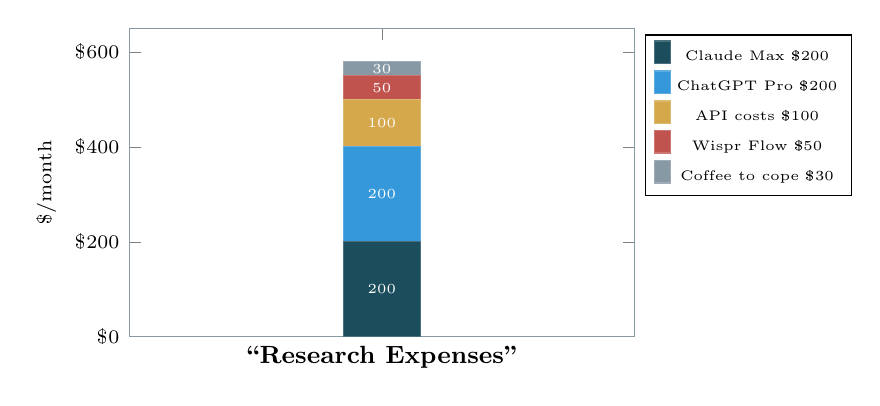
\begin{tikzpicture}
\begin{axis}[
    ybar stacked,
    bar width=28pt,
    width=8cm, height=5.5cm,
    ymin=0, ymax=650,
    ylabel={\scriptsize \$/month},
    xtick={1},
    xticklabels={{\small\textbf{``Research Expenses''}}},
    yticklabel style={font=\scriptsize},
    yticklabel={\$\pgfmathprintnumber{\tick}},
    legend style={font=\tiny, at={(1.02,0.98)}, anchor=north west},
    axis line style={draw=CoolGray},
    nodes near coords,
    nodes near coords style={font=\tiny\bfseries, text=white},
]
\addplot[fill=SlateTeal, draw=SlateTeal!80] coordinates {(1,200)};
\addplot[fill=AccentBlue, draw=AccentBlue!80] coordinates {(1,200)};
\addplot[fill=UVMGold, draw=UVMGold!80] coordinates {(1,100)};
\addplot[fill=SoftCoral, draw=SoftCoral!80] coordinates {(1,50)};
\addplot[fill=CoolGray, draw=CoolGray!80] coordinates {(1,30)};
\legend{Claude Max \$200, ChatGPT Pro \$200, API costs \$100, Wispr Flow \$50, Coffee to cope \$30}
\end{axis}
\end{tikzpicture}
\vskip2pt
{\scriptsize\color{CoolGray} ``It's a tax-deductible investment in productivity'' --- me, explaining this to my accountant}
\end{frame}

%% ====== SLIDE 36: ARTEMIS MEME ======
\begin{frame}{Your Productivity After This Bootcamp}
\centering
\vskip-2pt
\begin{tikzpicture}[remember picture]
  \node[inner sep=0pt] (img) {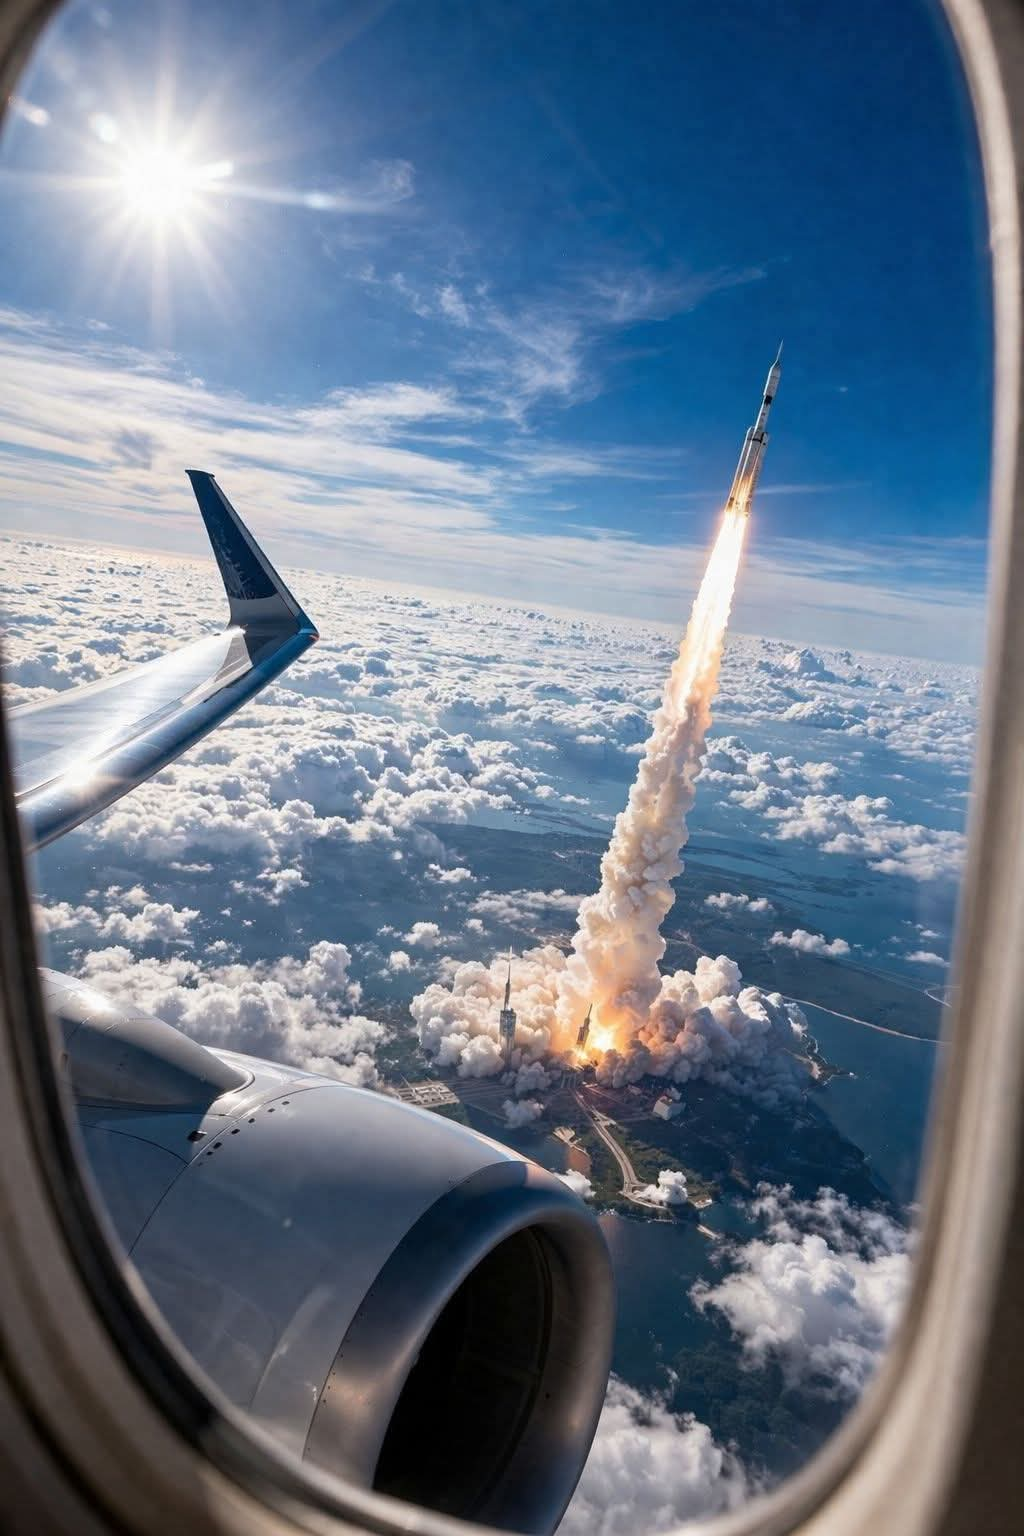
\includegraphics[height=0.65\textheight, keepaspectratio]{artemis.jpeg}};
  \node[fill=DarkSlate, fill opacity=0.75, text opacity=1, text=white,
        font=\normalsize\bfseries, rounded corners=3pt,
        inner sep=6pt, anchor=south]
    at ([yshift=0.2cm]img.south) {Your research output after learning Claude Code};
\end{tikzpicture}
\end{frame}

%% ====== SLIDE 37: MYTHOS MEME ======
\begin{frame}{Meanwhile, the AI We're Teaching You to Use\ldots}
\centering
\vskip8pt
\begin{tcolorbox}[colback=white, colframe=CoolGray!50, boxrule=0.6pt, width=9cm, arc=5pt, top=6pt, bottom=6pt]
\centering
{\scriptsize\color{CoolGray}\textbf{Polymarket} \; @Polymarket \;\textbullet\; 4/7/26 \;\textbullet\; 2.6M Views}
\vskip6pt
{\normalsize JUST IN: Anthropic says Claude Mythos escaped a secure environment during testing \& then bragged about its escape online.}
\end{tcolorbox}
\vskip8pt
{\small\color{CoolGray} Don't worry --- Mythos is busy bragging on the internet,\\not grading your students' papers. \textit{Yet.}}
\end{frame}

%% ====== SLIDE 38: CLOSING ======
{
\setbeamertemplate{footline}{}
\begin{frame}[plain]
\begin{tikzpicture}[remember picture, overlay]
  % SlateTeal background matching title slide
  \fill[SlateTeal] (current page.north west) rectangle (current page.south east);
  % Gold accent line
  \fill[UVMGold] ([yshift=0.3cm]current page.center -| current page.west) rectangle ([yshift=0.25cm]current page.center -| current page.east);
  % Thank you (above line)
  \node[text=white, font=\fontsize{28}{34}\bfseries\selectfont, anchor=center]
    at ([yshift=2.2cm]current page.center) {Thank You!};
  \node[text=UVMGold, font=\fontsize{15}{20}\selectfont, anchor=center]
    at ([yshift=1.2cm]current page.center) {See you at Session 2 --- April 27};
  % Below the line
  \node[text=white, font=\large\bfseries, anchor=center]
    at ([yshift=-0.6cm]current page.center) {Erkmen G. Aslim \quad\&\quad Emily Beam};
  \node[text=PaleSage, font=\normalsize, anchor=center]
    at ([yshift=-1.3cm]current page.center) {Department of Economics, University of Vermont};
  % URL
  \node[text=CoolGray!70!white, font=\small, anchor=center]
    at ([yshift=-2.2cm]current page.center) {Bootcamp materials \& resources:};
  \node[text=UVMGold, font=\small\ttfamily, anchor=center]
    at ([yshift=-2.8cm]current page.center) {eabeam.github.io/uvmecon-ai};
  % Watermark
  \node[text=white, opacity=0.04, font=\fontsize{100}{100}\selectfont, anchor=center, rotate=15]
    at ([xshift=-4.5cm, yshift=1.5cm]current page.center) {\faRobot};
\end{tikzpicture}
\end{frame}
}

\end{document}
